\documentclass{article} % For LaTeX2e
\usepackage{nips13submit_e,times}
\usepackage{hyperref}
\usepackage{algorithmic}
\usepackage{algorithm}
\usepackage{url}
\usepackage{amsmath}
\usepackage{mwe}
\usepackage{graphicx}
\usepackage{booktabs}
\usepackage{subfig}
\usepackage{tabularx}
\usepackage{epstopdf}
\usepackage{bm}
%\documentstyle[nips13submit_09,times,art10]{article} % For LaTeX 2.09



% The \author macro works with any number of authors. There are two commands
% used to separate the names and addresses of multiple authors: \And and \AND.
%
% Using \And between authors leaves it to \LaTeX{} to determine where to break
% the lines. Using \AND forces a linebreak at that point. So, if \LaTeX{}
% puts 3 of 4 authors names on the first line, and the last on the second
% line, try using \AND instead of \And before the third author name.

\newcommand{\fix}{\marginpar{FIX}}
\newcommand{\new}{\marginpar{NEW}}

\nipsfinalcopy % Uncomment for camera-ready version

\usepackage[english]{babel}
\usepackage[utf8x]{inputenc}
\usepackage{amsmath}
\usepackage[colorinlistoftodos]{todonotes}

\title{Decision making in 2-arm bandit problem}
\author{Hannah Chen \\
  \texttt{hechen@eng.ucsd.edu} \and \textbf{Sonali Rahagude}\\
  \texttt{srahagud@ucsd.edu} \and \textbf{Sneha Venkatesh Yelimeli}\\
  \texttt{svyelime@eng.ucsd.edu} \and \textbf{Chun Fan}\\
  \texttt{c9fan@ucsd.edu} \and \textbf{Yashodhan Karandikar}\\
  \texttt{ykarandi@eng.ucsd.edu}}

\date{\today}

\begin{document}
\maketitle

\begin{abstract}
%\todo[inline]{ADD ABSTRACT}
\end{abstract}

\section{Introduction}


\section{Background}
\label{background}

\section{Design}
\label{design}


\subsection{Environments}

\subsection{Generation of Optimal data}
\subsubsection{Formulation of MDP}
\todo[inline] {states definition, recursive formulation, decision rule}

\subsubsection{Algorithm}



\subsection{Inference of Parameters for Heuristics}
For inferring parameters for different heuristic methods, we use the optimal data and do a grid search. 

\subsubsection{$\epsilon$-greedy}

\subsubsection{$\epsilon$-decreasing}

\subsubsection{Win Stay Loose Shift}

\subsubsection{$\tau$-Switch}


\subsubsection{Common Algorithm Input : (alpha, beta, decisions, rewards), output: (parameter value)}
\label{appendixAlgo}
\begin{algorithm}[H]
\caption{LDA Generative process with collapsed Gibbs Sampling }
\label{generativeLDA_algorithm}
\renewcommand{\algorithmicrequire}{\textbf{Input:}}
\renewcommand{\algorithmicensure}{\textbf{Output:}}
\begin{algorithmic}[1]
		\REQUIRE words $\bm{w} \in $ documents $\bm{d} \in [1,D]$
%		\BEGIN \\
			\STATE randomly initialize $\bm{z}$ and increment counters
		\FOR {iteration $i \in [1,epoch]$}
			\FOR { document $d \in [1,D]$}
				\FOR {word $\in [1, N_{d}] $}
					\STATE $topic \leftarrow z[word]$
					\STATE decrement counters according to document $d$, $topic$ and $word$
					\FOR {$k \in [1,K]$}
						\STATE calculate $p(z=k|.) $ using Gibbs equation
					\ENDFOR
					\STATE $newTopic \leftarrow $ sample from $p(z|.)$
					\STATE $z[word] \leftarrow newTopic$
					\STATE decrement counters according to document $d$, $newTopic$ and $word$
				\ENDFOR
			\ENDFOR
		\ENDFOR
%		\END \\	
\end{algorithmic}
\end{algorithm}
	

%\section{Implementation}
\label{implementation}



\section{Results}
\label{results}

\subsection{Comparison with optimal data}

\begin{figure}[H]
\begin{center}
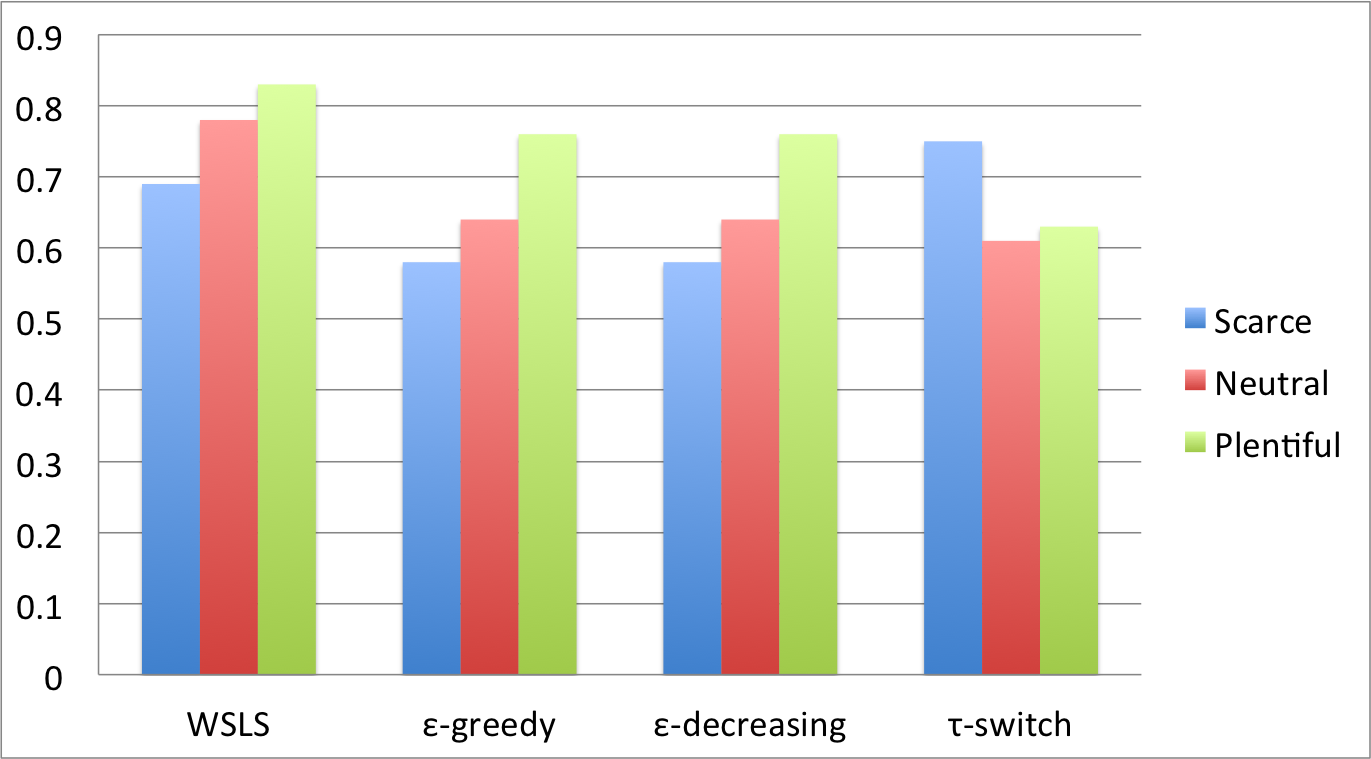
\includegraphics[scale=0.5]{optimalVsHeuristicNoTitle}
\caption{\small \sl \label{plot1} Agreement of Heuristic Models with Optimal Model}
\end{center}
\end{figure}

Figure~\ref{plot1} shows the agreement of each of the heuristic models with the decisions obtained using the optimal model, for each of the three environment settings. The agreement with optimal is maximum for the `plentiful' environment for most of the heuristics, which agrees with the results in the original paper.

\subsection{Comparison with human data}
\begin{figure}[H]
\begin{center}
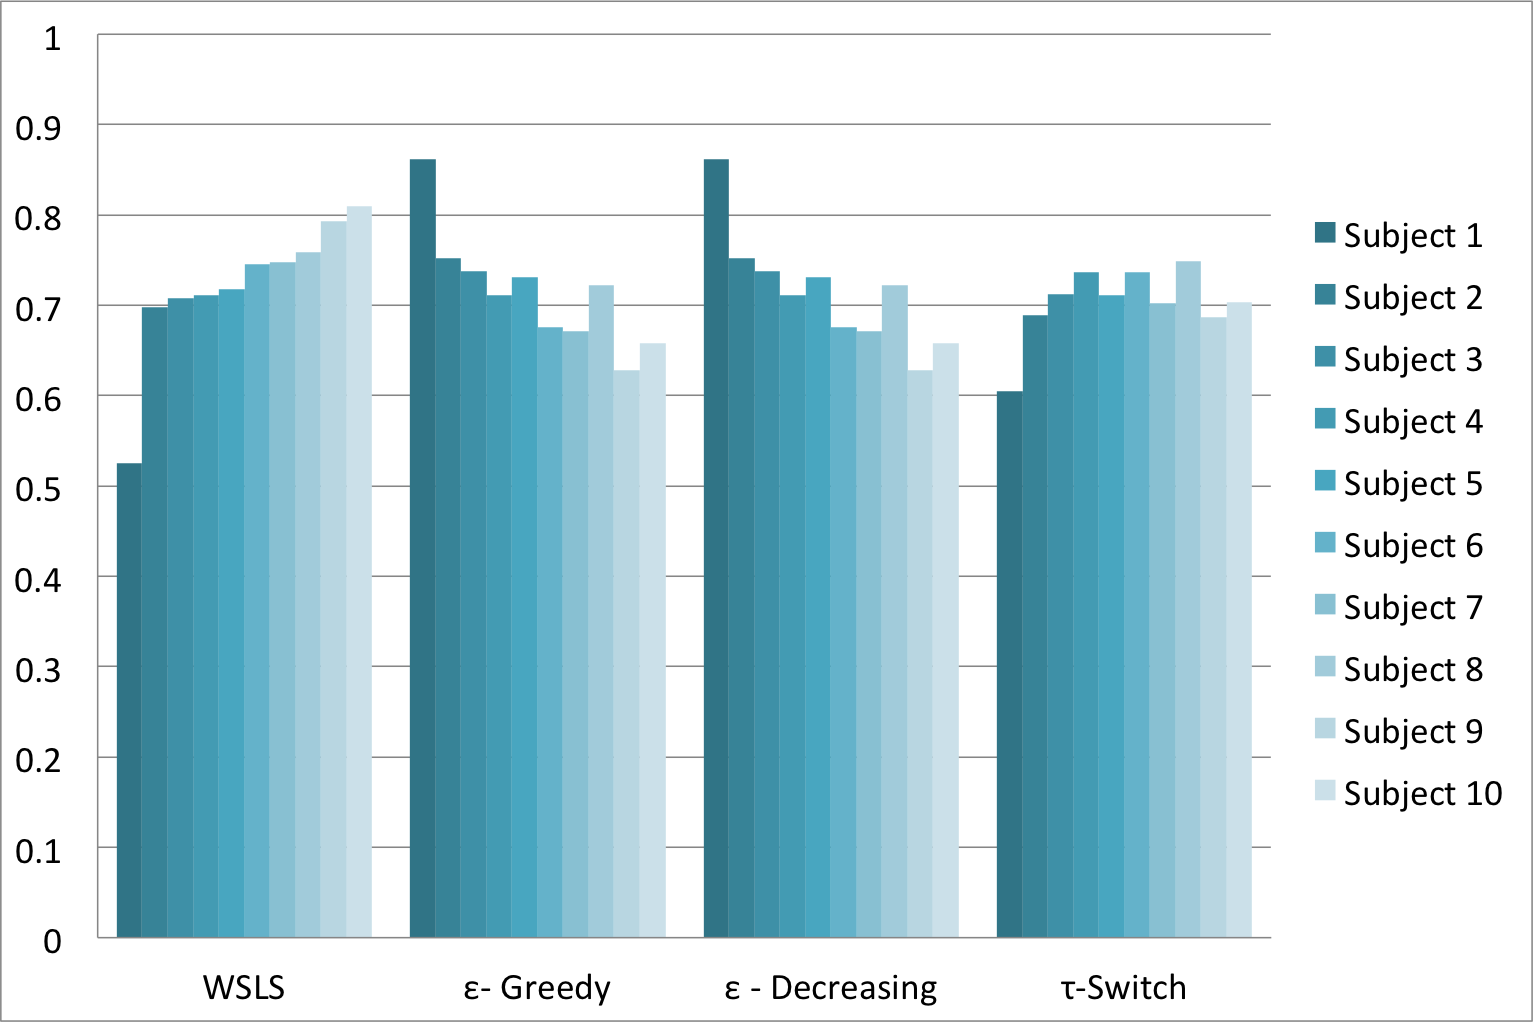
\includegraphics[scale=0.5]{humanVsHeuristicNoTitle}
\caption{\small \sl \label{plot2} Agreement of Heuristic Models with Human Data}
\end{center}
\end{figure}

Figure~\ref{plot2} shows the agreement of the heuristics with the human data for each of the 10 subjects. The 10 bars for the WSLS have been sorted in increasing order of agreement, while the bars for the remaining heuristics follow this sorted order of the participants.

\section{Conclusions}
\label{conclusions}
The project consisted of 3 goals: generating optimal data for different environments, and evaluating agreement of different heuristic models and the $\tau-switch$ model with the optimal data as well as the given human data. The first step was to understand how different environments can be obtained by different parameter settings of the beta distribution $Beta(\alpha, \beta)$ and then implementing sampling rewards for the optimal model. The decisions and rewards obtained from the optimal model make intuitive sense, depending on the prior confidence in the environment ($\alpha + \beta$), and expected rate of the rewards ($\alpha/ (\alpha + \beta)$). We found that our implementation does agree with the results of the paper \cite{shunan2011} to some extent. The fact that we use a different comparison metric (match percentage) instead of posterior predictive agreement used in \cite{shunan2011} might be the reason for the differences. 

\appendix
\section{Appendix}

\bibliography{bib}{}
\bibliographystyle{unsrt}


\end{document}